\section{KNN}
this chapter will give information on the classification method called KNN (K nearest neighbour).\\
the KNN classification will need a dataset often refereed to as the training data, the data in the training set has to be notated so one can know what is in the dataset. When one has the training data set they need some value because even though notated they can still be different, for this one can make use of different features to describe these differences. then the training data can be see as being scattered out on a field based on what value they have from the feature. now when there comes a new input, the input can be given a value from the features. then with the placement of the new data it needs to be named for that it can look at its neighbours to seen what it is similar to that is the nearest neighbour part, the K then will tell how many neighbours that has to be look at before determining what the new input is. 
\begin{figure}[h]
	\begin{center}
		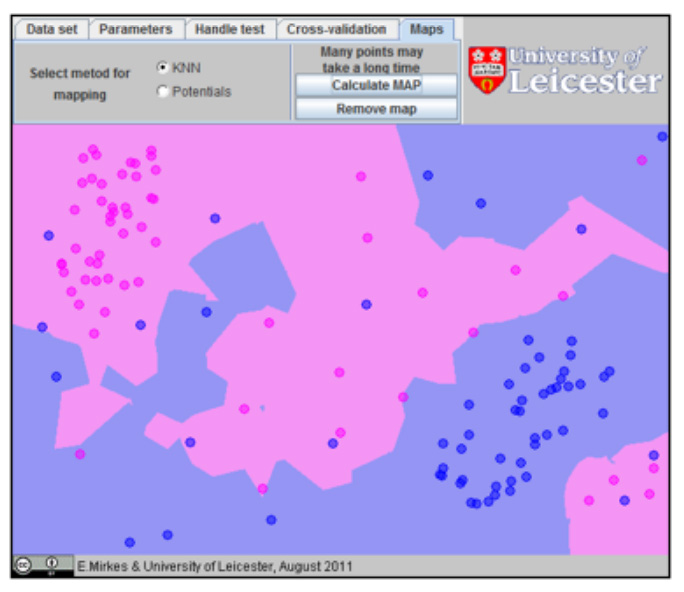
\includegraphics[scale = 0.5]{fig/KNNfig.jpg}
		\caption{KNN field here one can see how the knn will divide the space up with to different classes}
		\label{KNN fig}
	\end{center}
\end{figure}